%%%%%%%%%%%%%%%%%%%%%%%%%%%%%%%%%%%%%%%%%%%%%%%%%%%%%%%%%%%%%%%%%%
\subsection{Redes Neuronales Artificiales (\acrshort{ann})}
\label{sec:ann}

Antes de entrar en detalle en la optimización de hiperparámetros de la \gls{ann}, se debe indicar que esta Sección se divide en dos fases diferenciadas: primero, se centra la aplicación del método \textit{Grid Search} sobre el modelo de \gls{mlp} proporcionado por la librería \textit{sklearn} y, después, los resultados obtenidos de la búsqueda  se utilizan para configurar una nueva \gls{ann} optimizada, basada en el módulo \textit{keras}. Esta secuencia de pasos se establece a modo de simplificar la comprensión y de justificar y comparar los resultados que se obtienen para ambas versiones de \gls{ann}s.

\subsubsection{Optimización de hiperparámetros y ejecución del modelo de \acrshort{ann} de \textit{sklearn}}

En primera instancia, se determinan los hiperparámetros que se van a estudiar del \gls{mlp}. Estos hacen referencia a la configuración de capas ocultas y al número de neuronas que puede tener cada capa (\textit{hidden\_layer\_sizes}), a la función de activación que se aplica (\textit{activation}) y al algoritmo de optimización de los pesos de la red durante el proceso de entrenamiento (\textit{solver}). \cite{mlp}

\vspace{3mm}

\begin{lstlisting}[style=Python, caption={Cuadrícula de parámetros MLP}]
  param_grid = {
    'hidden_layer_sizes': [(5,), (8,), (10,), (50,), (100,), (5, 5), (8, 8), (10, 10), (50, 50)],  
    'activation': ['relu', 'tanh'],
    'solver': ['sgd', 'adam']
  }
\end{lstlisting}

\vspace{3mm}

En este caso, se configura para la búsqueda un modelo por defecto de \gls{mlp}, en el que se aplican un máximo de 100 iteraciones por cada combinación a probar. De la misma forma, para no introducir latencias innecesarias ni un sobreentrenamiento que perjudique a los resultados de clasificación, se determina una finalización temprana del entrenamiento cuando se produzcan una cantidad de iteraciones seguidas sin mejoras significativas. En este caso, se deja el valor por defecto, que es 10 iteraciones y se modifica la tolerancia a un valor de 0.00001.

\vspace{3mm}

\begin{lstlisting}[style=Python, caption={Clasificador MLP por defecto}]
  mlp = MLPClassifier(max_iter=100, verbose=True, early_stopping=True, tol=0.00001)
\end{lstlisting}

\vspace{3mm}

La creación del objeto de la clase \textit{GridSearchCV()}, con una configuración de 5 pliegues (\textit{cv=5}), y su entrenamiento sobre el \gls{mlp} anterior en un equipo de 32 procesadores, se estima en una duración de 2,34 horas. Cuando se lleva a cabo este proceso, se puede comprobar en el diccionario de resultados (\textit{cv\_results\_}) y, en particular, en los valores de precisión de la variable \textit{mean\_test\_score}, que el empleo del algoritmo de optimización del gradiente descendiente estocástico (\gls{sgd}) aporta mejores resultados que el \textit{adam}. 

\vspace{3mm}

En la Tabla \ref{tab:mlpaccuracy} se pueden encontrar varias combinaciones de hiperparámetros que optimizan el rendimiento, con un valor de precisión del 97,6\%. Sin embargo, también es importante poner el foco en los valores de desviación típica que se consiguen y en la duración del entrenamiento que supone cada opción para determinar cuál es la combinación de hiperparámetros más adecuada para el \gls{mlp}. 

\pagebreak

En el caso de la desviación típica, como se observa en la Tabla \ref{tab:mlpstd}, no se producen grandes diferencias de valores entre las configuraciones en cuestión, por lo que, a priori, no es un factor determinante a tener en cuenta en la selección. No obstante, en el caso de los tiempos sí existen variaciones, las cuales se deben al número de iteraciones que son necesarias para alcanzar la convergencia para cada versión de \gls{mlp} y a la duración que supone cada iteración. 

\vspace{3mm}

En la Tabla \ref{tab:mlptiempo}, se puede visualizar que, cuanto mayor sea el número de neuronas especificado, mayor será la latencia introducida. Esto presenta también, cierta correlación con los valores de la Tabla \ref{tab:mlpaccuracy}, ya que cuando el proceso de entrenamiento es relativamente largo, es posible que se produzca un sobreentrenamiento o \textit{overfitting} del modelo de \gls{mlp} y que la precisión obtenida sea más baja. Por ello, es importante configurar la tolerancia de optimización de forma correcta y detener el entrenamiento cuando se detecte la convergencia del modelo (\textit{early stopping}).

\vspace{3mm}

Por lo tanto, tras analizar los resultados, se expone de forma concluyente que la combinación de hiperparámetros más adecuada y que debería ser la configurada en el modelo de \gls{mlp}, es la que determina una estructura de dos capas ocultas de 5 neuronas, una función de activación \textit{relu} y el algoritmo de optimización \gls{sgd}. En este caso, como se puede apreciar en las Figuras \ref{fig:1mlpbestacc} y \ref{fig:1mlpbestloss} el proceso de entrenamiento converge en la iteración 41 con una precisión del 97,66\% y una función de pérdidas con valor 0,0712.

\vspace{3mm}

\begin{table}[H]
    \centering
    \begin{tabular}{|
    >{\columncolor[HTML]{EFEFEF}}c |cc|cc|}
    \hline
    \textit{Solver} & \multicolumn{2}{c|}{\cellcolor[HTML]{EFEFEF}\textit{adam}} & \multicolumn{2}{c|}{\cellcolor[HTML]{EFEFEF}\textit{sgd}} \\ \hline
    \textit{\begin{tabular}[c]{@{}c@{}}Función de activación /\\ Capas ocultas\end{tabular}} & \multicolumn{1}{c|}{\cellcolor[HTML]{EFEFEF}\textit{relu}} & \cellcolor[HTML]{EFEFEF}\textit{tanh} & \multicolumn{1}{c|}{\cellcolor[HTML]{EFEFEF}\textit{relu}} & \cellcolor[HTML]{EFEFEF}\textit{tanh} \\ \hline
    (5,) & \multicolumn{1}{c|}{90,17} & \multicolumn{1}{c|}{97,61} & \multicolumn{1}{c|}{97,66} & \multicolumn{1}{c|}{97,54} \\ \hline
    (8,) & \multicolumn{1}{c|}{92,03} & \multicolumn{1}{c|}{89,73} & \multicolumn{1}{c|}{97,65} & \multicolumn{1}{c|}{97,65} \\ \hline
    (10,) & \multicolumn{1}{c|}{87,00} & \multicolumn{1}{c|}{89,90} & \multicolumn{1}{c|}{97,48} & \multicolumn{1}{c|}{89,76} \\ \hline
    (50,) & \multicolumn{1}{c|}{86,89} & \multicolumn{1}{c|}{89,82} & \multicolumn{1}{c|}{89,53} & \multicolumn{1}{c|}{97,65} \\ \hline
    (100,) & \multicolumn{1}{c|}{90,95} & \multicolumn{1}{c|}{89,71} & \multicolumn{1}{c|}{84,56} & \multicolumn{1}{c|}{89,72} \\ \hline
    (5, 5) & \multicolumn{1}{c|}{89,80} & \multicolumn{1}{c|}{89,72} & \multicolumn{1}{c|}{97,66} & \multicolumn{1}{c|}{97,65} \\ \hline
    (8, 8) & \multicolumn{1}{c|}{88,49} & \multicolumn{1}{c|}{89,72} & \multicolumn{1}{c|}{89,89} & \multicolumn{1}{c|}{97,65} \\ \hline
    (10, 10) & \multicolumn{1}{c|}{81,68} & \multicolumn{1}{c|}{89,70} & \multicolumn{1}{c|}{90,30} & \multicolumn{1}{c|}{97,65} \\ \hline
    (50, 50) & \multicolumn{1}{c|}{81,91} & \multicolumn{1}{c|}{82,04} & \multicolumn{1}{c|}{97,66} & \multicolumn{1}{c|}{89,73} \\ \hline
    \end{tabular}
    \caption{Resultados de precisión (\%) (\textit{mean\_test\_score}) extraídos del atributo \textit{cv\_results\_} del \acrshort{mlp}}
    \label{tab:mlpaccuracy}
\end{table}

\vspace{3mm}

\begin{table}[H]
    \centering
    \begin{tabular}{|
    >{\columncolor[HTML]{EFEFEF}}c |cc|cc|}
    \hline
    \textit{Solver} & \multicolumn{2}{c|}{\cellcolor[HTML]{EFEFEF}\textit{adam}} & \multicolumn{2}{c|}{\cellcolor[HTML]{EFEFEF}\textit{sgd}} \\ \hline
    \textit{\begin{tabular}[c]{@{}c@{}}Función de activación /\\ Capas ocultas\end{tabular}} & \multicolumn{1}{c|}{\cellcolor[HTML]{EFEFEF}\textit{relu}} & \cellcolor[HTML]{EFEFEF}\textit{tanh} & \multicolumn{1}{c|}{\cellcolor[HTML]{EFEFEF}\textit{relu}} & \cellcolor[HTML]{EFEFEF}\textit{tanh} \\ \hline
    (5,) & \multicolumn{1}{c|}{14,75} & \multicolumn{1}{c|}{0,10} & \multicolumn{1}{c|}{0,01} & \multicolumn{1}{c|}{0,22} \\ \hline
    (8,) & \multicolumn{1}{c|}{11,33} & \multicolumn{1}{c|}{15,84} & \multicolumn{1}{c|}{0,00} & \multicolumn{1}{c|}{0,00} \\ \hline
    (10,) & \multicolumn{1}{c|}{15,54} & \multicolumn{1}{c|}{15,51} & \multicolumn{1}{c|}{0,33} & \multicolumn{1}{c|}{15,78} \\ \hline
    (50,) & \multicolumn{1}{c|}{15,58} & \multicolumn{1}{c|}{15,74} & \multicolumn{1}{c|}{11,09} & \multicolumn{1}{c|}{0,00} \\ \hline
    (100,) & \multicolumn{1}{c|}{9,40} & \multicolumn{1}{c|}{15,90} & \multicolumn{1}{c|}{16,65} & \multicolumn{1}{c|}{15,87} \\ \hline
    (5, 5) & \multicolumn{1}{c|}{15,83} & \multicolumn{1}{c|}{15,87} & \multicolumn{1}{c|}{0,01} & \multicolumn{1}{c|}{0,00} \\ \hline
    (8, 8) & \multicolumn{1}{c|}{12,19} & \multicolumn{1}{c|}{15,87} & \multicolumn{1}{c|}{15,52} & \multicolumn{1}{c|}{0,00} \\ \hline
    (10, 10) & \multicolumn{1}{c|}{19,77} & \multicolumn{1}{c|}{15,89} & \multicolumn{1}{c|}{14,71} & \multicolumn{1}{c|}{0,00} \\ \hline
    (50, 50) & \multicolumn{1}{c|}{19,52} & \multicolumn{1}{c|}{19,20} & \multicolumn{1}{c|}{0,01} & \multicolumn{1}{c|}{15,85} \\ \hline
    \end{tabular}
    \caption{Resultados de desviación típica (\%) (\textit{std\_test\_score}) extraídos del atributo \textit{cv\_results\_} del \acrshort{mlp}}
    \label{tab:mlpstd}
\end{table}

\vspace{3mm}

\begin{table}[H]
    \centering
    \begin{tabular}{|
    >{\columncolor[HTML]{EFEFEF}}c |cc|cc|}
    \hline
    \textit{Solver} & \multicolumn{2}{c|}{\cellcolor[HTML]{EFEFEF}\textit{adam}} & \multicolumn{2}{c|}{\cellcolor[HTML]{EFEFEF}\textit{sgd}} \\ \hline
    \textit{\begin{tabular}[c]{@{}c@{}}Función de activación /\\ Capas ocultas\end{tabular}} & \multicolumn{1}{c|}{\cellcolor[HTML]{EFEFEF}\textit{relu}} & \cellcolor[HTML]{EFEFEF}\textit{tanh} & \multicolumn{1}{c|}{\cellcolor[HTML]{EFEFEF}\textit{relu}} & \cellcolor[HTML]{EFEFEF}\textit{tanh} \\ \hline
    (5,) & \multicolumn{1}{c|}{88} & \multicolumn{1}{c|}{37} & \multicolumn{1}{c|}{63} & \multicolumn{1}{c|}{35} \\ \hline
    (8,) & \multicolumn{1}{c|}{96} & \multicolumn{1}{c|}{43} & \multicolumn{1}{c|}{35} & \multicolumn{1}{c|}{36} \\ \hline
    (10,) & \multicolumn{1}{c|}{94} & \multicolumn{1}{c|}{40} & \multicolumn{1}{c|}{56} & \multicolumn{1}{c|}{43} \\ \hline
    (50,) & \multicolumn{1}{c|}{157} & \multicolumn{1}{c|}{168} & \multicolumn{1}{c|}{143} & \multicolumn{1}{c|}{70} \\ \hline
    (100,) & \multicolumn{1}{c|}{236} & \multicolumn{1}{c|}{223} & \multicolumn{1}{c|}{170} & \multicolumn{1}{c|}{131} \\ \hline
    (5, 5) & \multicolumn{1}{c|}{136} & \multicolumn{1}{c|}{50} & \multicolumn{1}{c|}{52} & \multicolumn{1}{c|}{44} \\ \hline
    (8, 8) & \multicolumn{1}{c|}{159} & \multicolumn{1}{c|}{54} & \multicolumn{1}{c|}{69} & \multicolumn{1}{c|}{46} \\ \hline
    (10, 10) & \multicolumn{1}{c|}{149} & \multicolumn{1}{c|}{55} & \multicolumn{1}{c|}{54} & \multicolumn{1}{c|}{48} \\ \hline
    (50, 50) & \multicolumn{1}{c|}{333} & \multicolumn{1}{c|}{319} & \multicolumn{1}{c|}{166} & \multicolumn{1}{c|}{155} \\ \hline
    \end{tabular}
    \caption{Resultados de tiempo (s) (\textit{mean\_fit\_time}) extraídos del atributo \textit{cv\_results\_} del \acrshort{mlp}}
    \label{tab:mlptiempo}
\end{table}

\vspace{3mm}

\begin{lstlisting}[style=Python, caption={Clasificador MLP óptimo}]
  mlp = MLPClassifier(max_iter=100, verbose=True, early_stopping=True, tol=0.00001, hidden_layer_sizes=(5, 5), activation='relu', solver='sgd')
\end{lstlisting}

\vspace{3mm}

\begin{figure}[H]
  \centering
  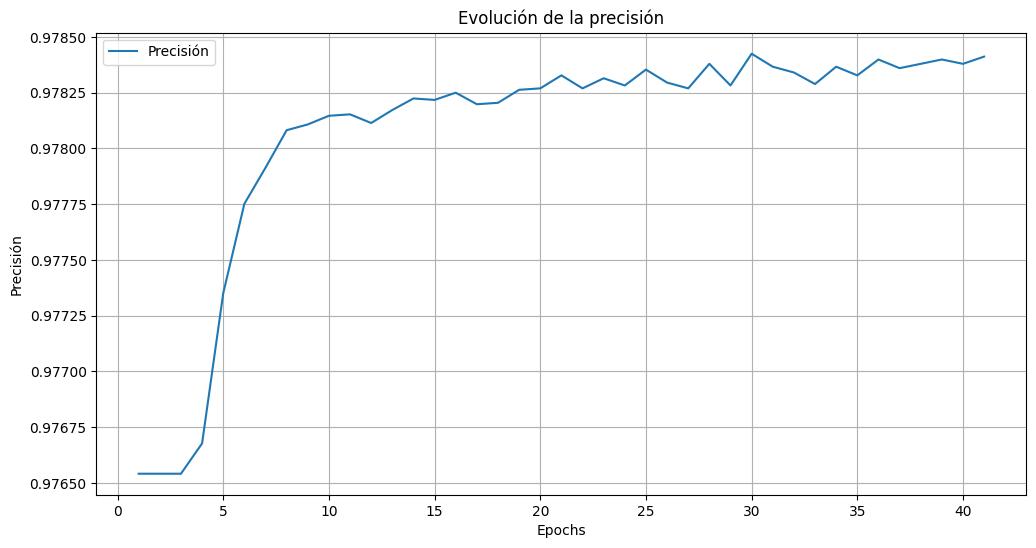
\includegraphics[width=1\textwidth]{img/desarrollo/ann/1mlpbestacc.png}
  \caption{Representación del valor de precisión en función de las iteraciones para el modelo de \acrshort{mlp} escogido}
  \label{fig:1mlpbestacc}
\end{figure}

\begin{figure}[H]
  \centering
  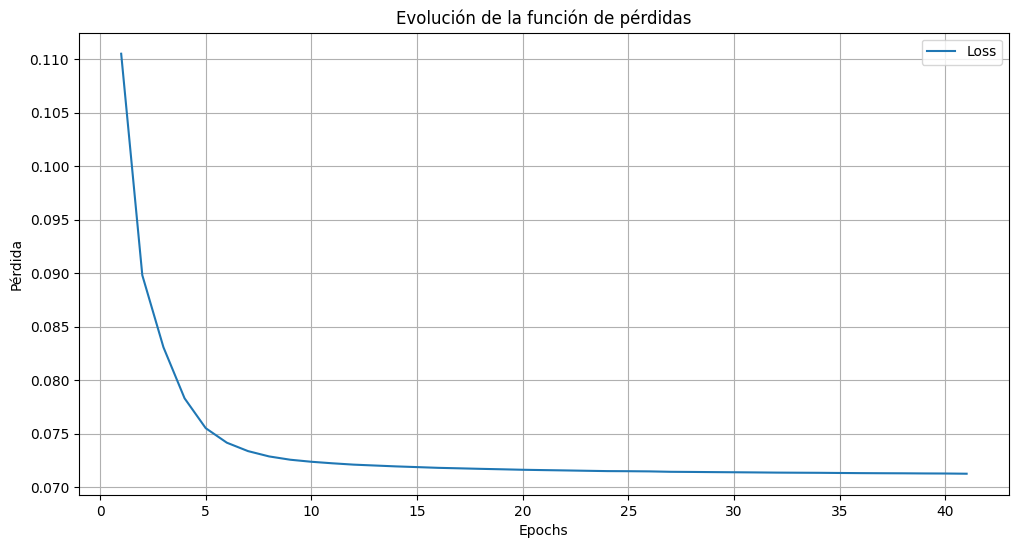
\includegraphics[width=1\textwidth]{img/desarrollo/ann/1mlpbestloss.png}
  \caption{Representación del valor de la función de pérdidas en función de las iteraciones para el modelo de \acrshort{mlp} escogido}
  \label{fig:1mlpbestloss}
\end{figure}

\subsubsection{Ejecución del modelo de \acrshort{ann} de \textit{keras} y evaluación de resultados}

Una vez seleccionada la combinación de hiperparámetros que produce un rendimiento óptimo del \gls{mlp}, el siguiente paso consiste en aplicar la configuración en cuestión a un nuevo modelo de \gls{ann}. El objetivo es realizar una comparativa entre dos \gls{ann}s proporcionadas por distintas librerías, como son en este caso \textit{sklearn} y el módulo \textit{keras} de \textit{tensorflow}, y comprobar que los resultados obtenidos de aplicar el método \textit{Grid Search} anteriormente son coherentes. 

\vspace{3mm}

Por ello, se define la estructura del modelo de \gls{ann} de \textit{keras} con las dos capas ocultas de 5 neuronas y una capa de una neurona a la salida, puesto que se trabaja con un conjunto de datos con etiquetas binarias. Además, es necesario especificar a la entrada el número de características (\textit{input\_shape}), ya que será igual al número de entradas de la red neuronal. La estructura del modelo definido se representa gráficamente en la Figura \ref{fig:neuronas} mediante el uso de la herramienta online proporcionada por \textit{TensorFlow}. \cite{seq}

\vspace{3mm}

\begin{lstlisting}[style=Python, caption={Definición del modelo de ANN de Keras}]
  model = keras.Sequential([
    keras.layers.Dense(5, input_shape=(X.shape[1],), activation='relu'), 
    keras.layers.Dense(5, activation='relu'),
    keras.layers.Dense(1, activation='sigmoid') 
  ]) 
\end{lstlisting}

\vspace{3mm}

\begin{figure}[H]
  \centering
  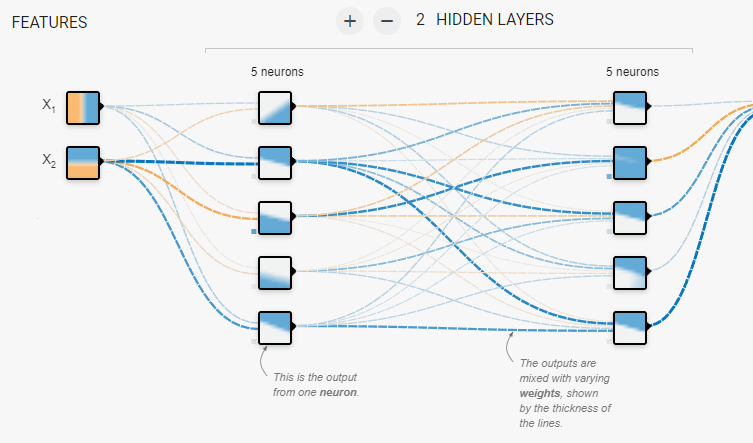
\includegraphics[width=0.9\textwidth]{img/desarrollo/ann/neuronas.png}
  \caption{Representación de la estructura de capas de la \gls{ann} \cite{tensorflow}}
  \label{fig:neuronas}
\end{figure}

\vspace{3mm}

Por consiguiente, se compila la red configurando el algoritmo de optimización \gls{sgd}. También, la función de pérdidas binaria (\textit{binary\_crossentropy}), cuyo valor vendrá dado por la entropía cruzada media entre los positivos que se predicen y los que realmente lo son. Después, se inicia el entrenamiento para un total de 100 iteraciones y se activa la finalización temprana del proceso, en el caso de acontecer 10 iteraciones seguidas sin mejoras significativas (0.00001) en la función de pérdidas. \cite{early}

\vspace{3mm}

\begin{lstlisting}[style=Python, caption={Entrenamiento del modelo de ANN de Keras}]
  model.compile(optimizer = 'sgd', loss = 'binary_crossentropy', metrics = ['accuracy'])
  History = model.fit(X_train, y_train, epochs=100, verbose=1, callbacks=[keras.callbacks.EarlyStopping(monitor='val_loss', patience=10, verbose=1, min_delta=0.00001)])
\end{lstlisting}

\vspace{3mm}

De la misma forma que en el modelo anterior, se almacenan los valores de precisión y de pérdidas de cada iteración y se representan en forma de gráfica lineal en las Figuras \ref{fig:3annacc} y \ref{fig:3annloss}. Como se puede ver, en este caso el entrenamiento del modelo de \gls{ann} de \textit{keras} no finaliza antes de llegar a las 100 iteraciones como ocurría con el \gls{mlp}. Sin embargo, los valores de la función de pérdidas y de precisión que se adquieren son muy similares respecto al modelo anterior, siendo de 0,068 y del 97,87\%, respectivamente. 

\vspace{3mm}

Una vez se han definido y entrenado los dos modelos de \gls{ann} anteriores, se introduce una etapa final de evaluación y validación mediante dos técnicas. Por un lado, se aplica la matriz de confusión, al igual que se realizaba para los modelos de \gls{ml} y, por otro lado, se hace empleo de los propios métodos de evaluación que ofrecen ambas \gls{ann}s. Como en esta Sección enfocada al \gls{dl} no se lleva a cabo una etapa de selección de características, la evaluación se ciñe a la comparación de resultados de ambos modelos de \gls{ann}s. 

\vspace{3mm}

En la Tabla \ref{tab:anncm}, se puede apreciar la similitud de los resultados, obteniéndose un mismo valor de precisión global (\textit{Accuracy}) para los dos modelos implementados (97,84\%). No obstante, si se pone el foco en el resto de métricas, se percibe una efectividad en la detección de errores (\textit{Recall}) ligeramente mayor para la \gls{ann} de \textit{sklearn} (14,98\%), mientras que
la \gls{ann} de \textit{keras} produce una mayor confiabilidad (\textit{Precision}) y, por tanto, una menor probabilidad de falsos positivos (72,17\%). 

\vspace{3mm}

Por consiguiente, en la Tabla \ref{tab:anneval} se exponen los resultados de aplicar los métodos \textit{score} y \textit{evaluate}, proporcionados por \textit{sklearn} y \textit{keras}, respectivamente. En el primer caso, solo se puede obtener el valor de precisión del modelo, mientras que en el segundo se aportan también las pérdidas. Como es de esperar, los resultados siguen siendo similares para ambas \gls{ann}s y, por tanto, se puede expresar que el estudio realizado en esta Sección es coherente. De forma concluyente, aunque las diferencias entre ambos modelos son mínimas, como se prioriza la efectividad en la detección de positivos, se escogería el modelo desarrollado con la librería \textit{keras}.

\vspace{3mm}

\begin{figure}[H]
  \centering
  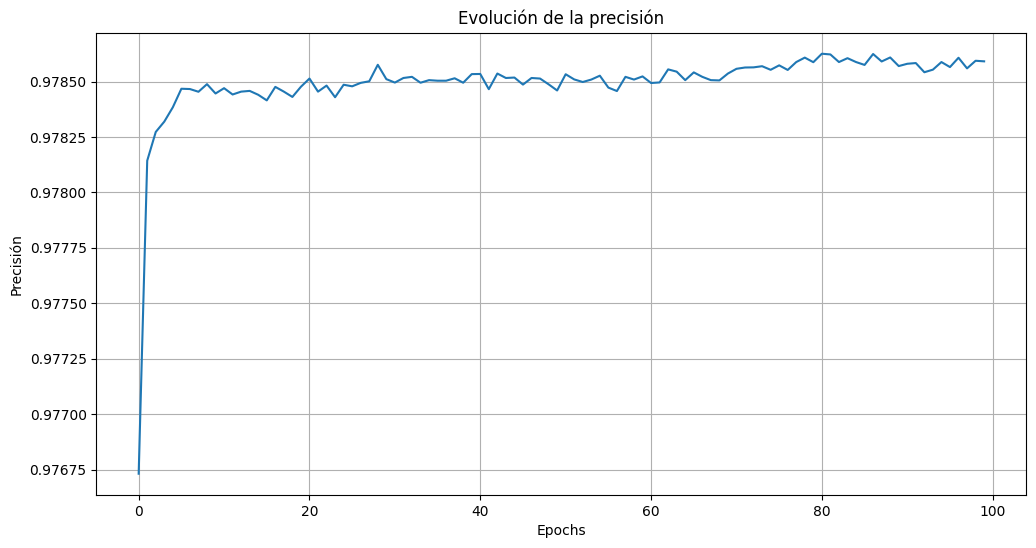
\includegraphics[width=1\textwidth]{img/desarrollo/ann/3annacc.png}
  \caption{Representación del valor de precisión en función de las iteraciones para el modelo de \acrshort{ann}}
  \label{fig:3annacc}
\end{figure}

\begin{figure}[H]
  \centering
  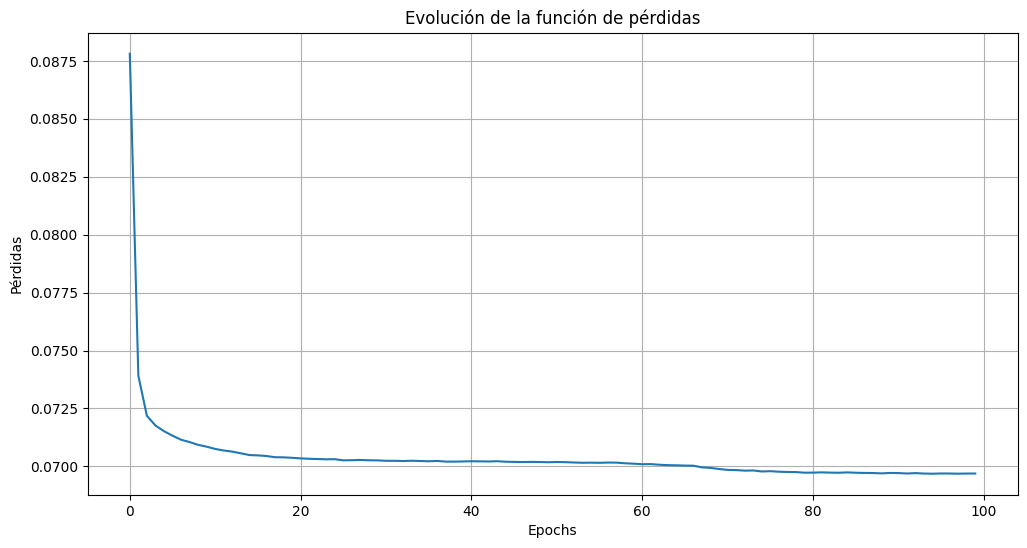
\includegraphics[width=1\textwidth]{img/desarrollo/ann/3annloss.png}
  \caption{Representación del valor de la función de pérdidas en función de las iteraciones para el modelo de \acrshort{ann}}
  \label{fig:3annloss}
\end{figure}

\vspace{3mm}

\begin{table}[H]
  \centering
  \begin{tabular}{|c|c|c|c|c|c|c|c|c|}
  \hline
  \rowcolor[HTML]{EFEFEF} 
  \textit{\begin{tabular}[c]{@{}c@{}}Matriz\\ de confusión\end{tabular}} & \cellcolor[HTML]{EFEFEF}\textit{TN} & \textit{FP} & \textit{FN} & \textit{TP} & \textit{Accuracy} & \textit{Precision} & \textit{Recall} & \textit{F1 Score} \\ \hline
  \cellcolor[HTML]{EFEFEF}\textit{sklearn} & 376535 & 609 & 7706 & 1358 & 97,84 & 69,03 & 14,98 & 24,66 \\ \hline
  \cellcolor[HTML]{EFEFEF}\textit{keras} & 376674 & 470 & 7842 & 1222 & 97,84 & 72,17 & 13,49 & 22,74 \\ \hline
  \end{tabular}
  \caption{Resultados de aplicación de la matriz de confusión a las \gls{ann}s}
  \label{tab:anncm}
\end{table}

\vspace{3mm}

\begin{table}[H]
  \centering
  \begin{tabular}{|c|c|c|c|c|c|c|c|c|}
  \hline
  \rowcolor[HTML]{EFEFEF} 
  \textit{\begin{tabular}[c]{@{}c@{}}Métodos propios de evaluación\end{tabular}} & \cellcolor[HTML]{EFEFEF}\textit{Accuracy} & \textit{Loss} \\ \hline
  \cellcolor[HTML]{EFEFEF}\textit{sklearn (score)} & 97,83 & - \\ \hline
  \cellcolor[HTML]{EFEFEF}\textit{keras (evaluate)} & 97,85 & 0,0690 \\ \hline
  \end{tabular}
  \caption{Resultados de aplicación de los métodos \textit{score} y \textit{evaluate} a las \gls{ann}s}
  \label{tab:anneval}
\end{table}

